% Likelihood scans with nuisance groups without the FSR cut
The extraction of the signal strength modifier $\mu$ proceeds throuth the maximisation of the likelyhood,
as described in Section~\ref{sec:statistical_analysis}.
This procedure can be visualised by scanning the likelihood function for several values of the parameter $\mu$ while profiling the nuisance parameters.
For each value the best fit value of the nuisance parameters is computed,
and the resulting value of the likelihood is stored.
These points are then plotted as a function of $\mu$.

Usually the auxiliary quantity $-2\Delta\text{ln}\Likelihood$ (defined as $t_0$ in Equation~\ref{eq:test_statistic})
is used instead of the likelihood itself.
The width of the its profile is linked to the uncertainty on the estimate of $\mu$ from the fit.
More precisely, the set of values ${ \mu / -2\Delta\text{ln}\Likelihood(\mu) < 1 (4) }$ corresponds to the 68\usep\% (95\usep\%) confidence interval.

This procedure can also be perfromed by fixing the values of one or more nuisances instead of allowing them to be fitted by the algorithm.
The effect of fixing the value of one or more parameters is a reduction in the width of the likelyhood shape.
This difference is ascribed to the effect of the frozen parameters.

\begin{figure}
  \centering
  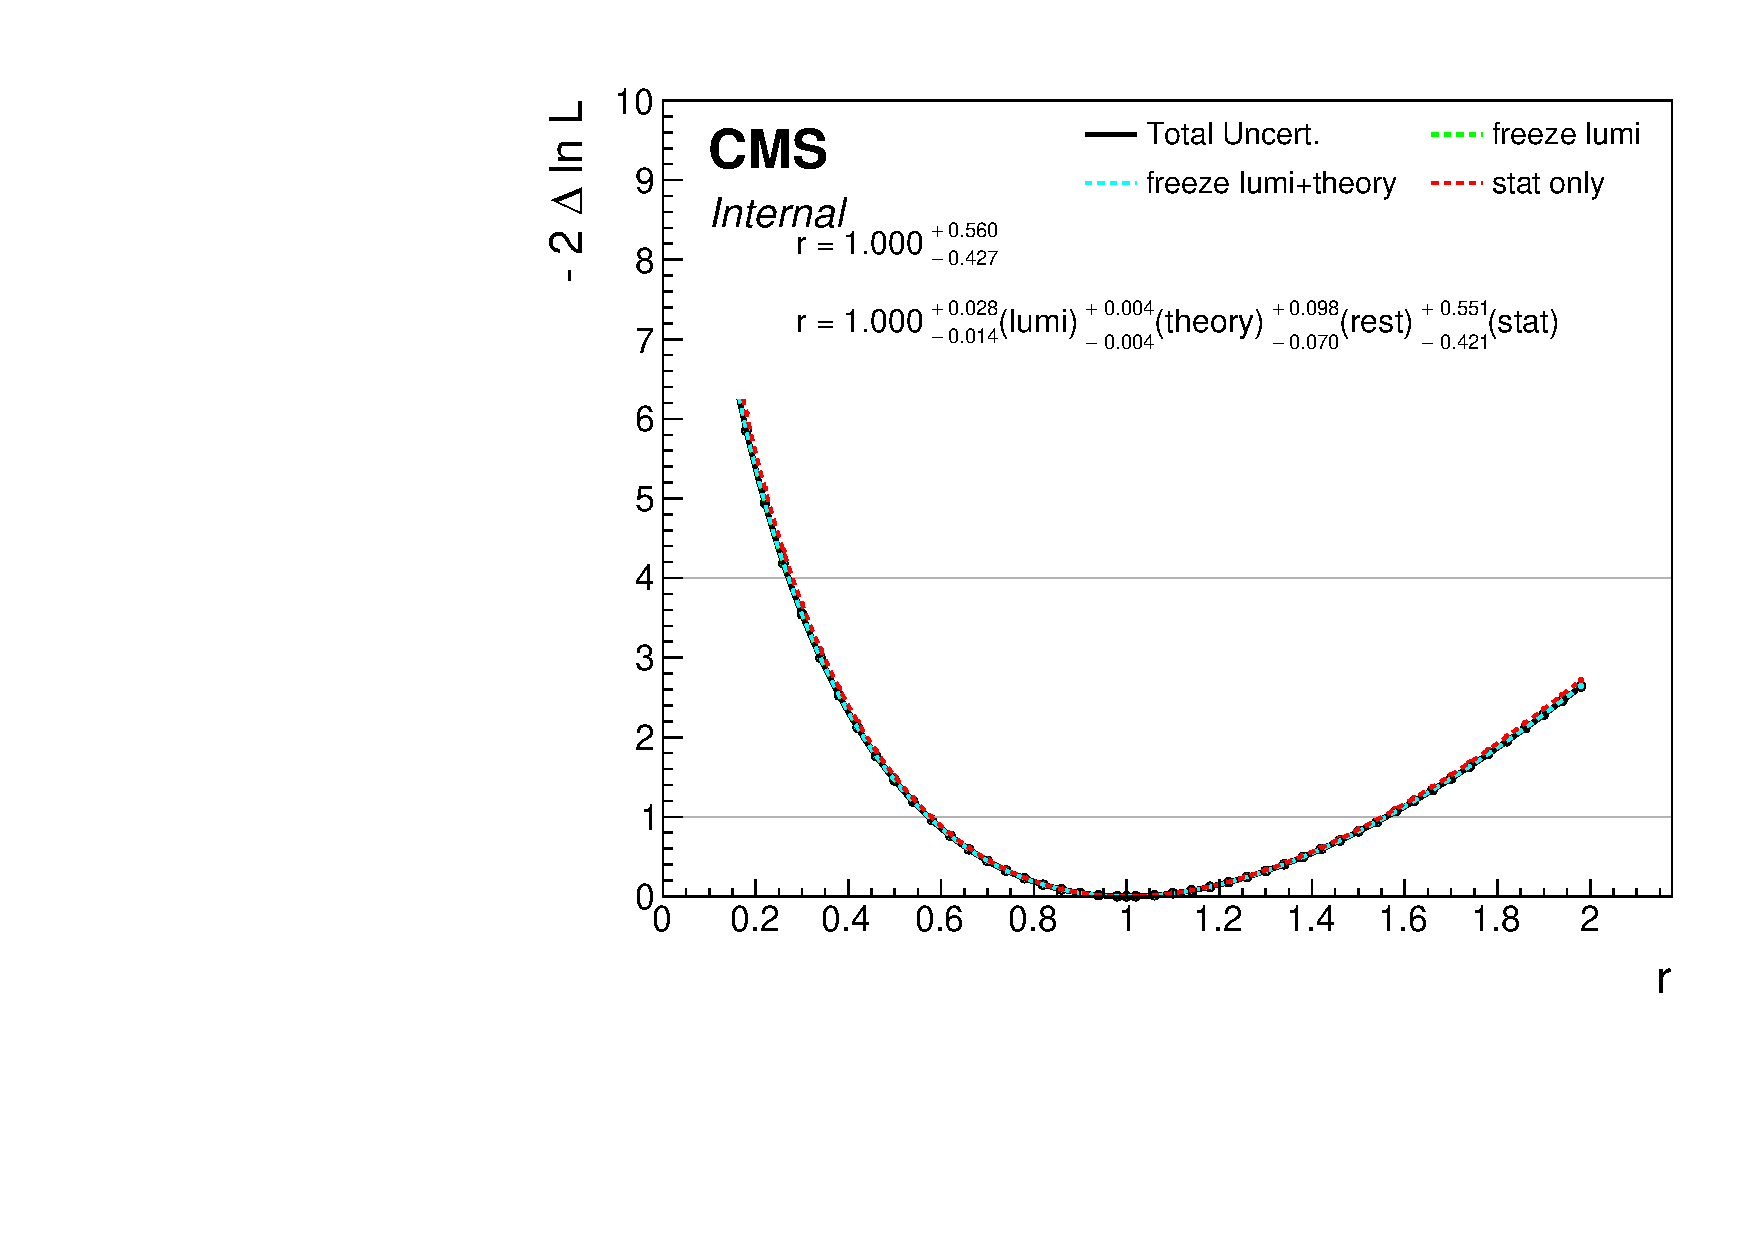
\includegraphics[height=.33\textheight]{scan_expected_Run2_SR4P_phoCR_lepCR_mZZGloose.pdf}
  \caption{Likelihood scan for the signal strength parameter
    on the mass of the $\PZ\PZ\PGg$ system,
    using the Loose working point of the photon cut-based ID.
    The data-driven estimate for \nonprompt photons is used.
    The FSR cut is not applied.
    The effect of groups of nusiance parameters on the uncertainty is assessed by sequentially fixing their value in the fit.
  }
  \label{fig:scan_Run2_SR4P_phoCR_lepCR_mZZGloose}
\end{figure}

\begin{figure}
  \centering
  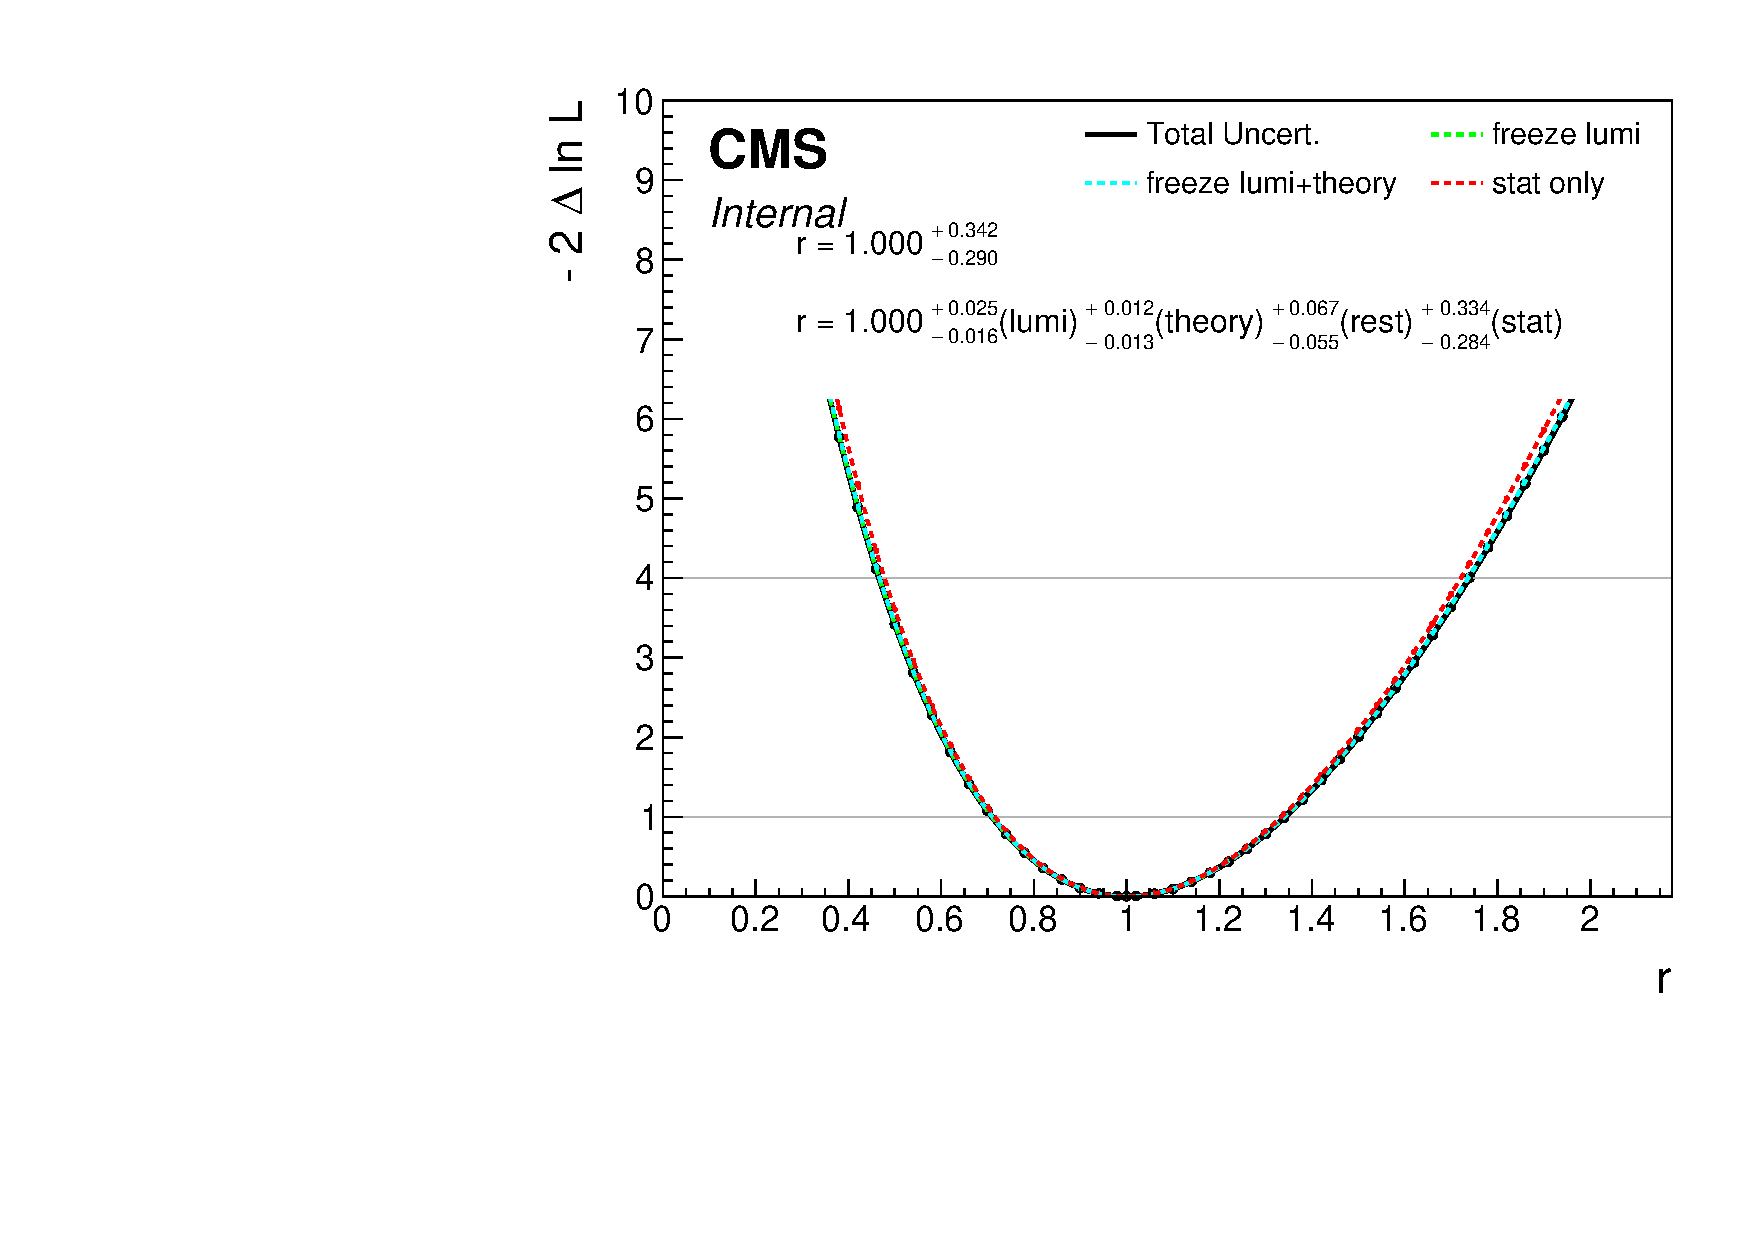
\includegraphics[height=.33\textheight]{scan_expected_Run2_SR4P_phoMC_lepCR_mZZGloose.pdf}
  \caption{Likelihood scan for the signal strength parameter
    on the mass of the $\PZ\PZ\PGg$ system,
    using the Loose working point of the photon cut-based ID.
    \Nonprompt photons are estimated from simulation.
    The FSR cut is not applied.
    The effect of groups of nusiance parameters on the uncertainty is assessed by sequentially fixing their value in the fit.
  }
  \label{fig:scan_Run2_SR4P_phoMC_lepCR_mZZGloose}
\end{figure}

\begin{figure}
  \centering
  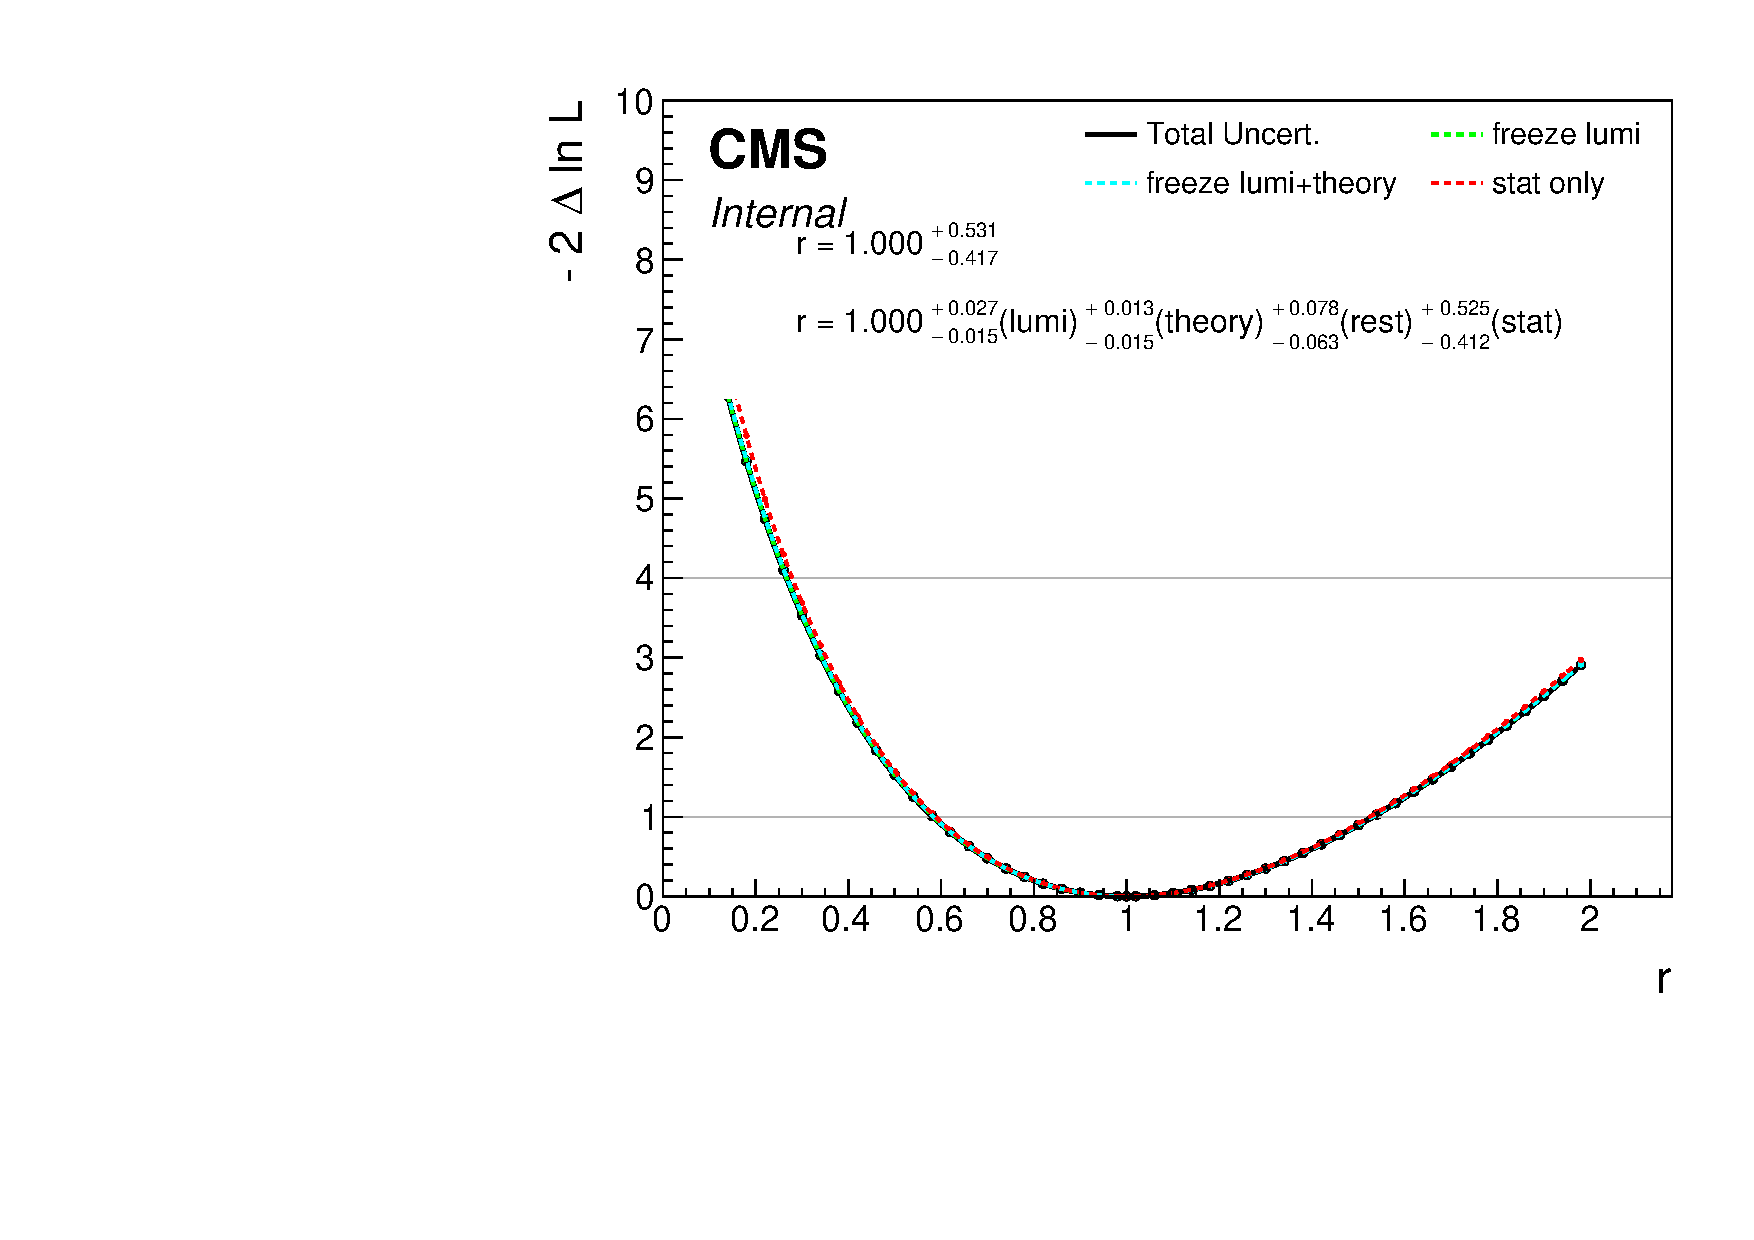
\includegraphics[height=.33\textheight]{scan_expected_Run2_SR4P_phoMC_lepCR_mZZGwp90.pdf}
  \caption{Likelihood scan for the signal strength parameter
    on the mass of the $\PZ\PZ\PGg$ system,
    using the \texttt{wp90} working point of the photon MVA ID.
    \Nonprompt photons are estimated from simulation.
    The FSR cut is not applied.
    The effect of groups of nusiance parameters on the uncertainty is assessed by sequentially fixing their value in the fit.
  }
  \label{fig:scan_Run2_SR4P_phoMC_lepCR_mZZGwp90}
\end{figure}

\begin{figure}
  \centering
  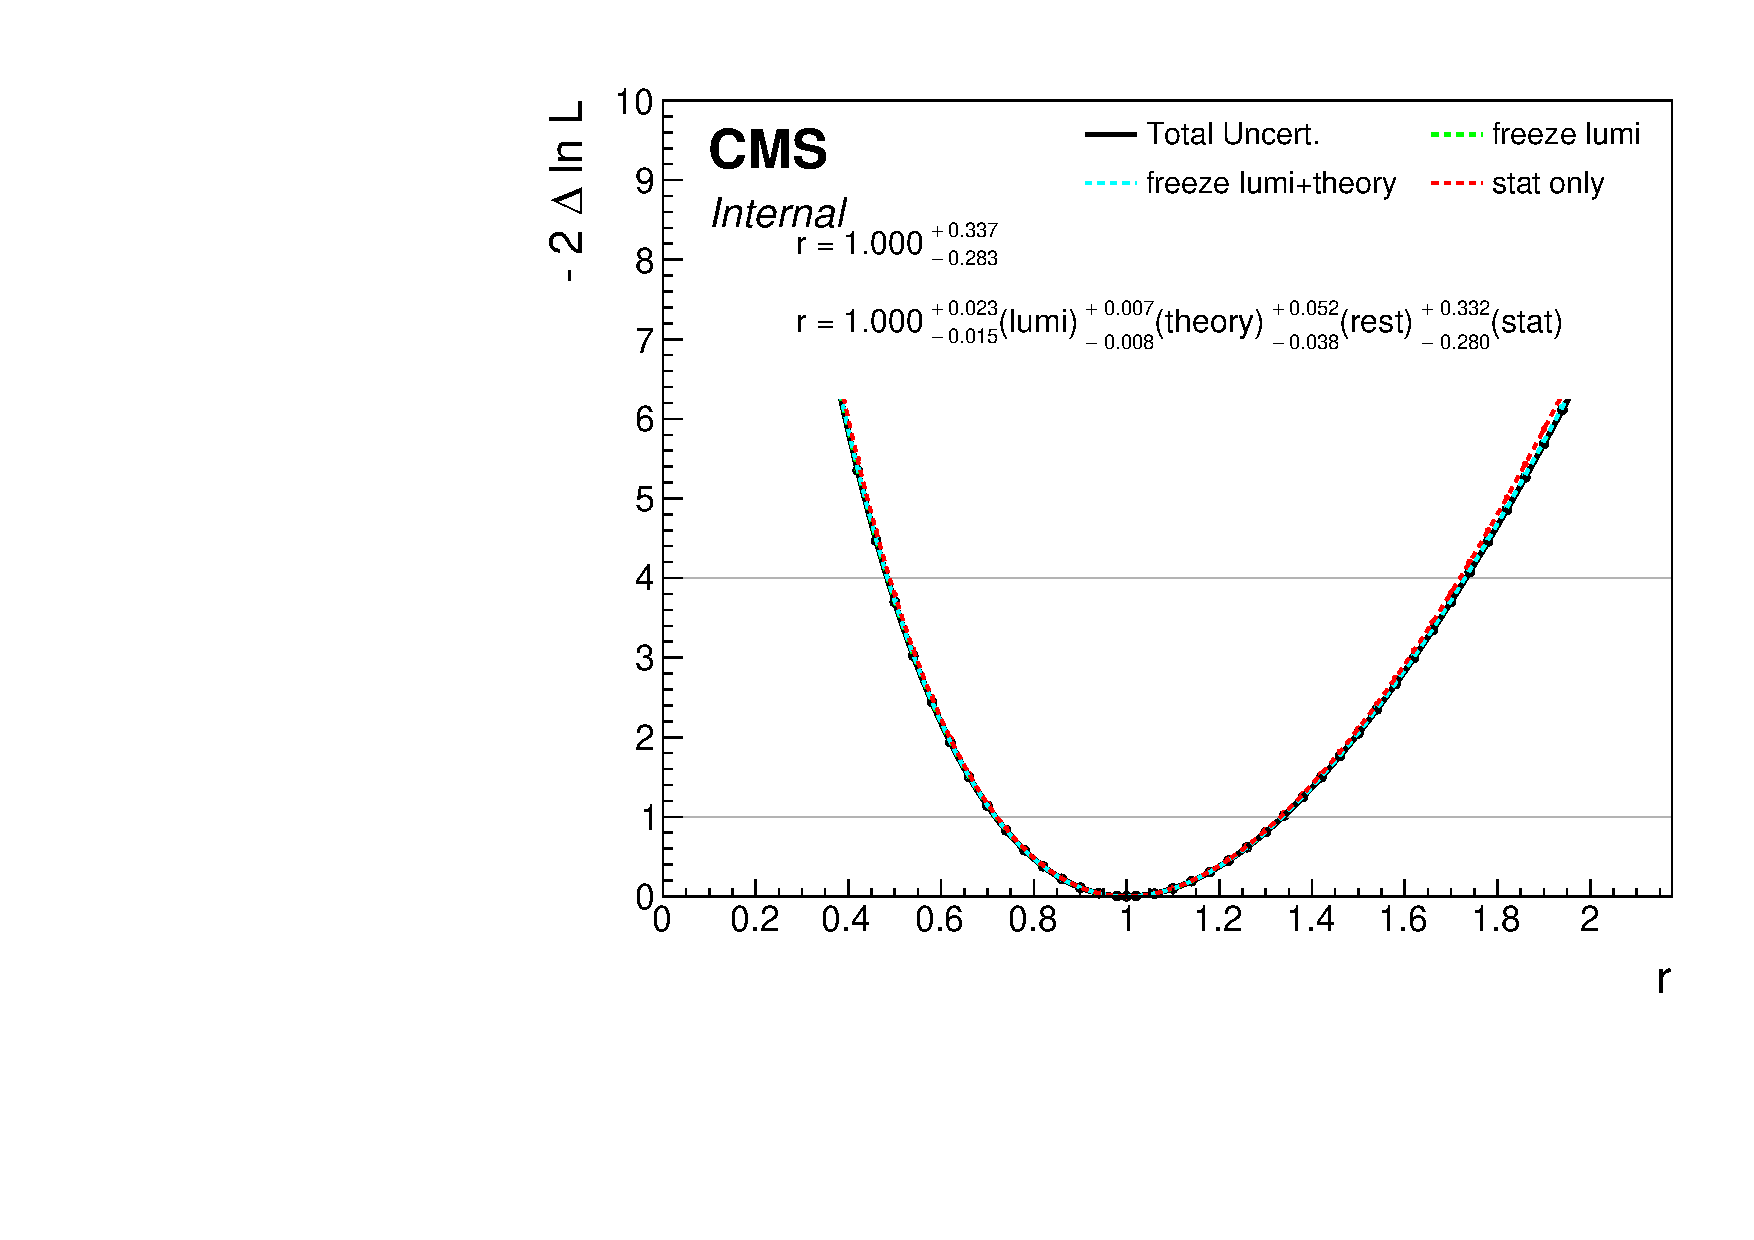
\includegraphics[height=.33\textheight]{scan_expected_Run2_SR4P_phoMC_lepCR_mZZGwp80.pdf}
  \caption{Likelihood scan for the signal strength parameter
    on the mass of the $\PZ\PZ\PGg$ system,
    using the \texttt{wp80} working point of the photon MVA ID.
    \Nonprompt photons are estimated from simulation.
    The FSR cut is not applied.
    The effect of groups of nusiance parameters on the uncertainty is assessed by sequentially fixing their value in the fit.
  }
  \label{fig:scan_Run2_SR4P_phoMC_lepCR_mZZGwp80}
\end{figure}

\begin{figure}
  \centering
  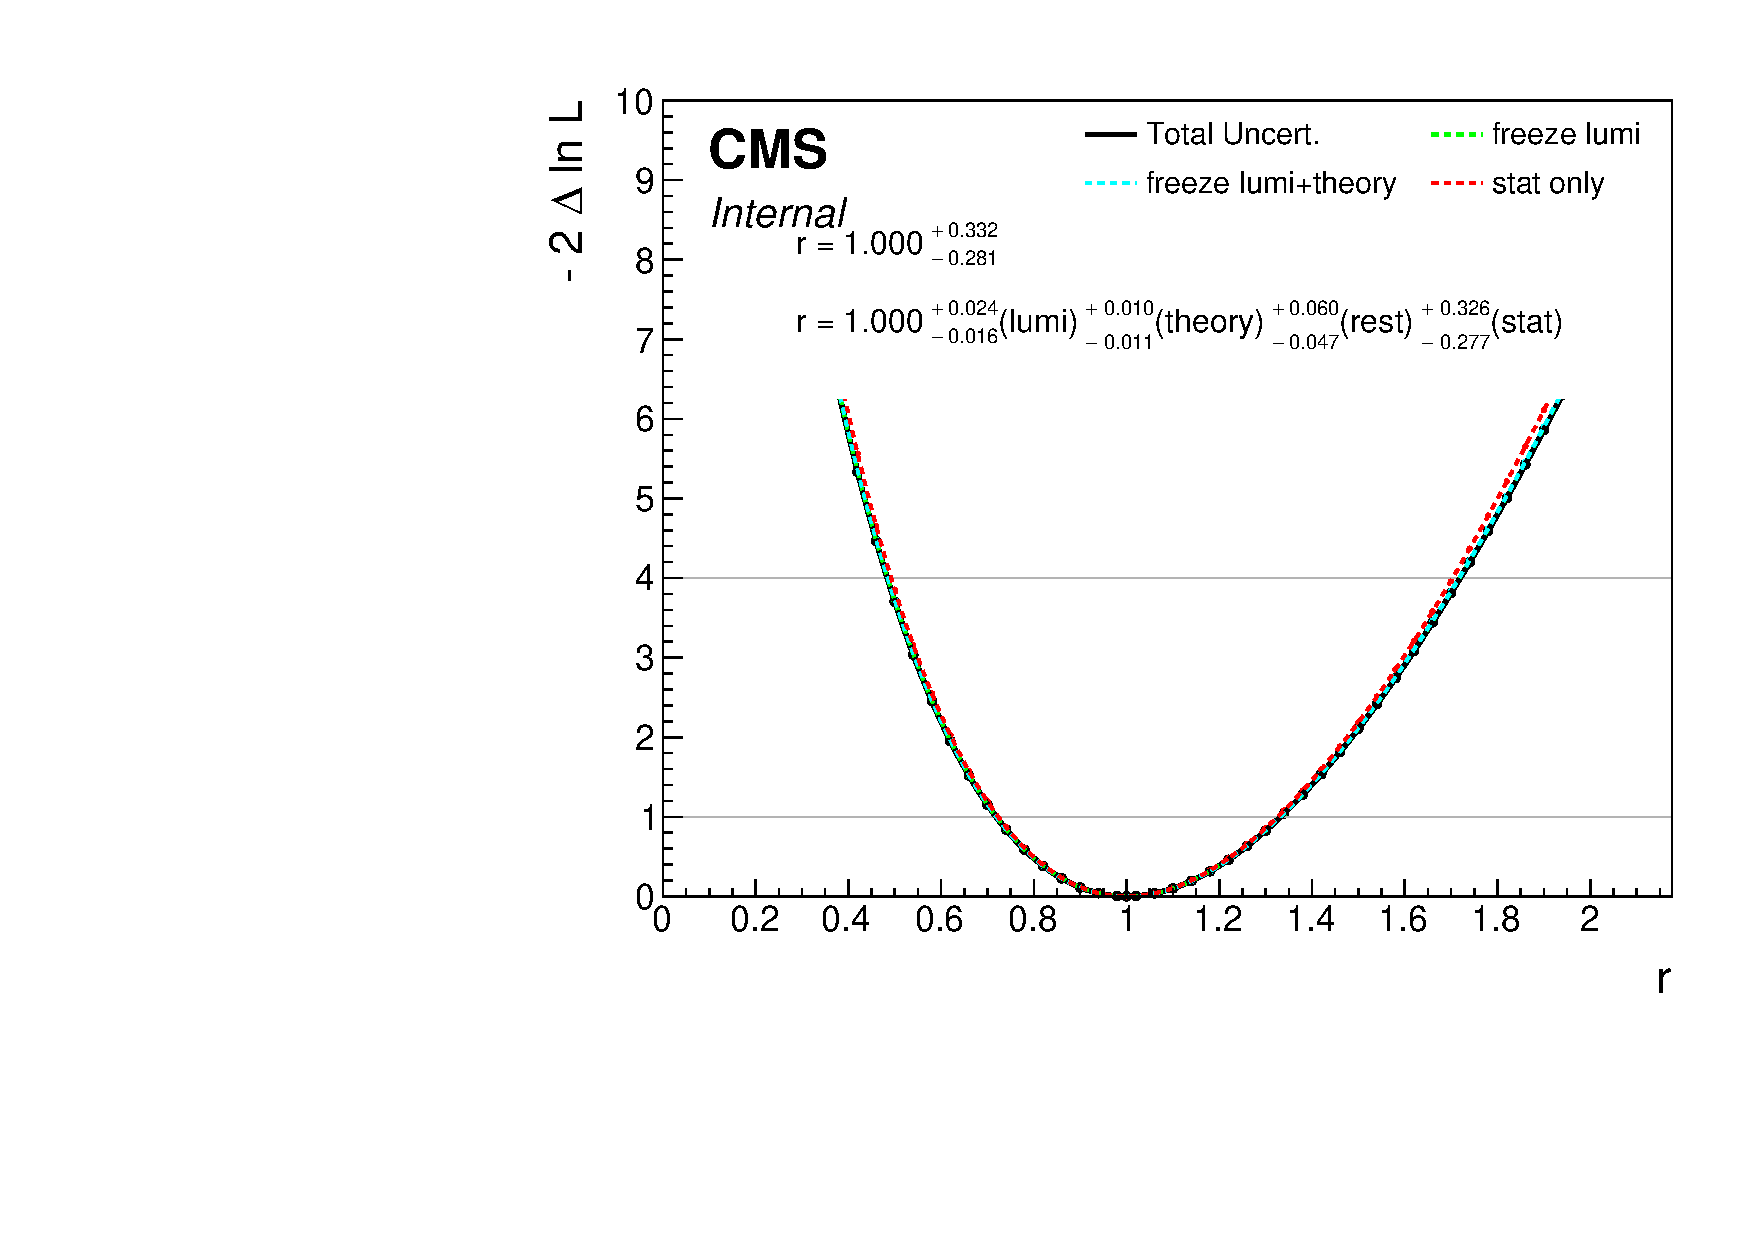
\includegraphics[height=.33\textheight]{scan_expected_Run2_SR4P_phoMC_lepCR_wp90pt.pdf}
  \caption{Likelihood scan for the signal strength parameter
    on the transverse momentum of the photon,
    using the \texttt{wp90} working point of the photon MVA ID.
    \Nonprompt photons are estimated from simulation.
    The FSR cut is not applied.
    The effect of groups of nusiance parameters on the uncertainty is assessed by sequentially fixing their value in the fit.
  }
  \label{fig:scan_Run2_SR4P_phoMC_lepCR_wp90pt}
\end{figure}

\begin{figure}
  \centering
  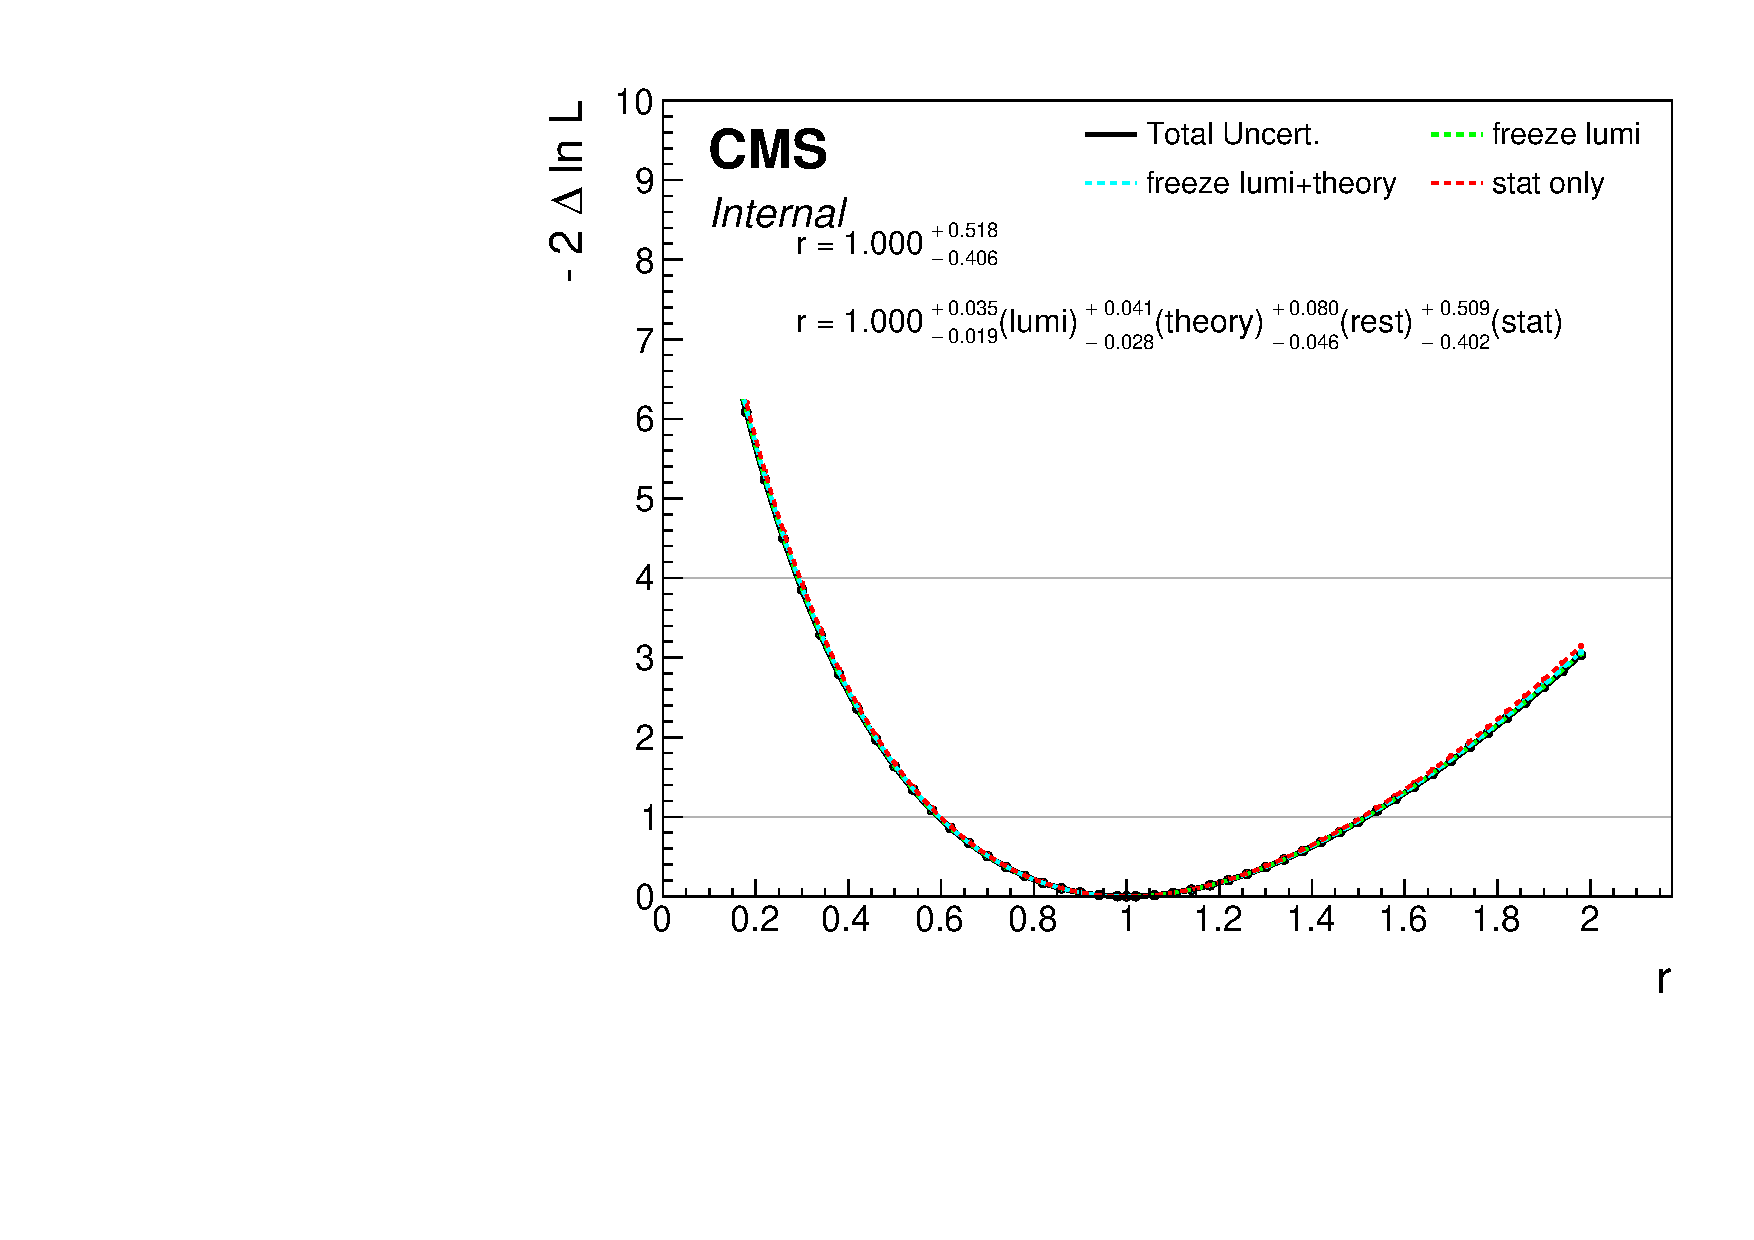
\includegraphics[height=.33\textheight]{scan_expected_Run2_SR4P_phoMC_lepCR_MVAcut.pdf}
  \caption{Likelihood scan for the signal strength parameter
    on the yield in the various bins of the photon MVA ID.
    \Nonprompt photons are estimated from simulation.
    The FSR cut is not applied.
    The effect of groups of nusiance parameters on the uncertainty is assessed by sequentially fixing their value in the fit.
  }
  \label{fig:scan_Run2_SR4P_phoMC_lepCR_MVAcut}
\end{figure}
